% 第四章 生成场景的质量验证
\chapter{生成场景的质量验证}
\section{实验设置}
\textbf{(1)测试数据集构成} \par
测试数据集旨在综合自动驾驶场景的多样性和复杂性,涵盖多种典型场景类别,如直行障碍、转弯障碍、变道、超车、闯红灯、无保护左转、右转、以及交叉路口协商等。这些场景类别覆盖了自动驾驶车辆在实际道路环境中可能遇到的关键交互情况,具备较高的代表性和实用价值。
数据集中的场景描述以自然语言形式呈现,且包括一定比例的模糊性描述,以模拟真实世界中驾驶员或其他交通参与者行为的不可预测性。场景描述的模糊性设计有助于测试生成系统在面对不精确指令时的处理能力,确保系统能够适应并生成符合要求的复杂交通场景。\\
\indent\textbf{(2)对比基线选择依据} \par
在评估生成场景的质量时,本研究选用了两种具有代表性的方法作为基线进行对比:
基于规则的方法(Rule-based):该方法通过定义明确的逻辑和规则来生成场景,具有较好的可解释性,适合处理结构化和预定义的任务。然而,在面对复杂和模糊的自然语言描述时,其灵活性和适应性较差。
基于GPT-4.0的方法:借助于大型语言模型的生成能力,能够生成丰富多样的场景。尽管其在场景生成的多样性方面具有优势,但可能在生成的场景物理合规性和逻辑一致性上存在一定不足,尤其是在处理复杂交通情境时。
选择这两种基线的目的是为了从不同角度评估本研究方法在生成场景质量、效率以及对复杂和模糊指令的鲁棒性方面的优势。\\
\indent\textbf{(3)硬件平台与评估指标} \par
硬件平台:本实验使用联想Y900P高性能笔记本电脑。该平台配置了多核的 Intel Core i9 处理器,能够高效处理复杂的计算任务,确保场景生成的实时性和响应速度。此外,配备的专业级显卡为图形处理和并行计算任务提供了强大支持,尤其是在大规模场景生成过程中。系统还配备大容量内存和高速固态硬盘(SSD),确保数据处理和存储高效、稳定。
评估指标:为了全面评估生成场景的质量,本研究采用以下几个关键指标:
场景生成时间:该指标衡量生成一个场景所需的时间,反映了系统的效率。较短的生成时间有助于提高测试的灵活性和响应速度。
场景物理合规性:评估生成场景是否符合物理约束条件,如车辆的最大加速度、最小转弯半径等。物理合规性确保了场景的真实性,生成的场景能真实反映自动驾驶系统的实际驾驶条件。
场景逻辑一致性:检查场景中各元素之间的逻辑关系是否合理,确保生成的场景符合法律规定的交通规则。逻辑一致性是验证场景真实性和可接受性的核心标准。
场景多样性:统计生成场景的类型和数量,衡量系统的多样性和生成能力。多样性高的系统能为自动驾驶系统提供更广泛的测试场景,从而有效覆盖更多潜在的驾驶情况。
碰撞率:在仿真环境中运行生成的场景,并统计发生碰撞的频率。碰撞率反映了生成场景的安全性,较低的碰撞率意味着生成的场景能够较好地模拟真实世界中的安全驾驶环境。




\section{生成效果展示(示例)}

\subsection{场景一:摩托车和汽车在红绿灯前等待信号}
\indent 一辆摩托车和一辆汽车在红绿灯前等待信号。\\

\begin{figure}[H]
	\centering
	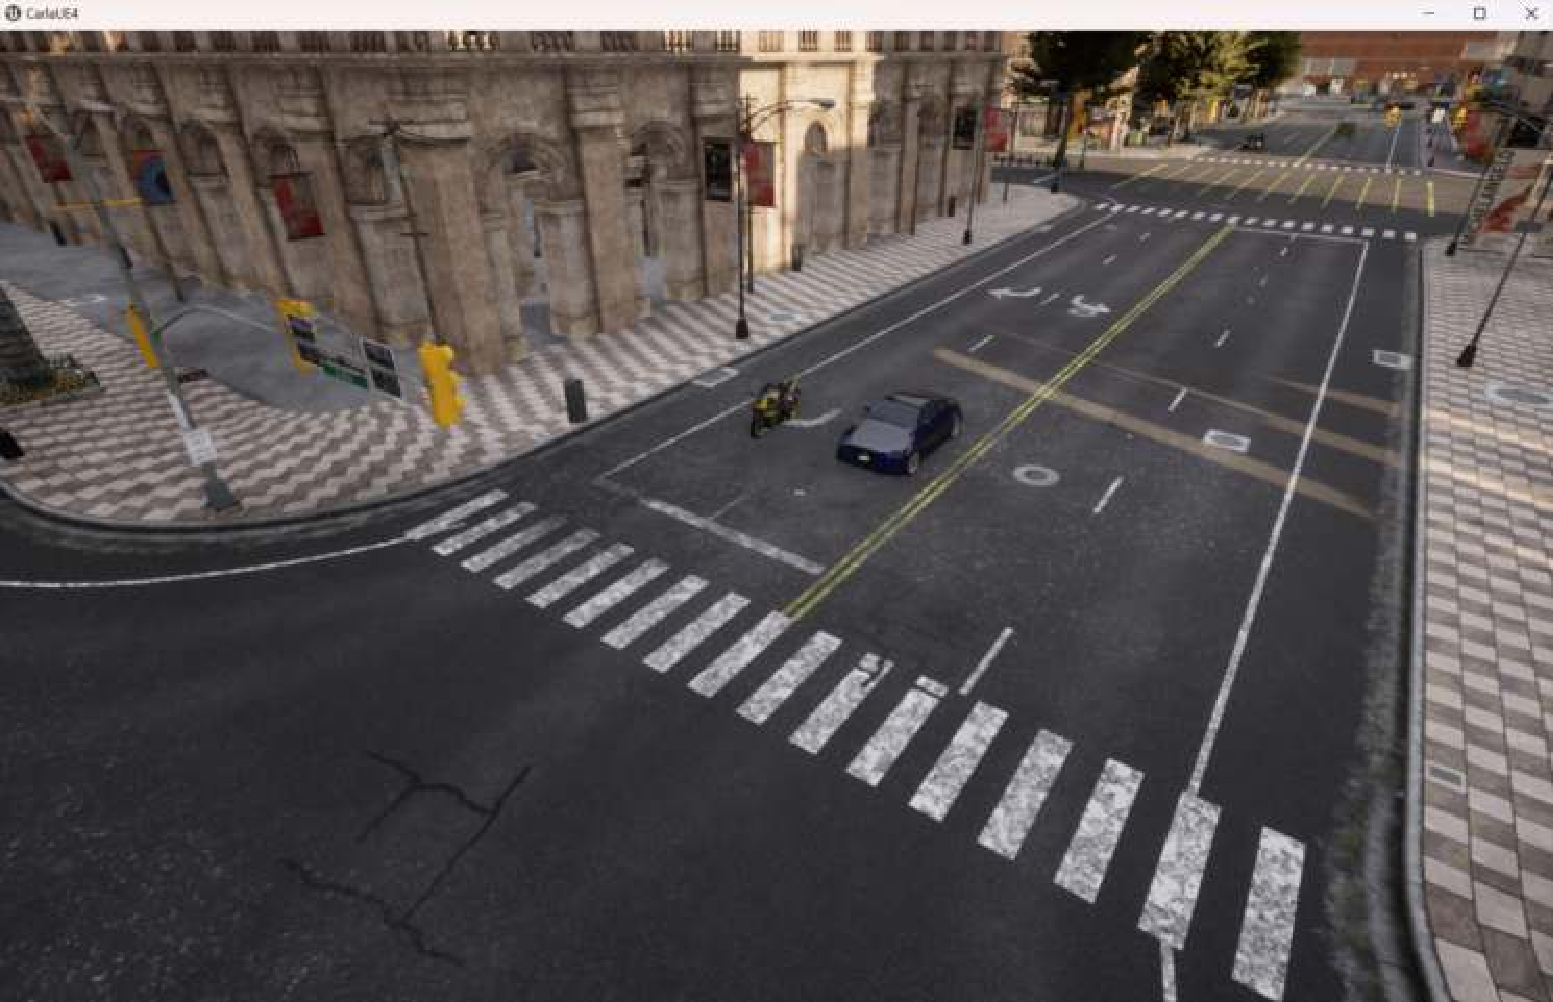
\includegraphics[width=0.7\textwidth]{"images/1.png"}
	\caption{摩托车与汽车在红绿灯前等待信号的场景截图}
	\label{fig:redlight_motorbike_car}
\end{figure}

\subsection{场景二:自我车辆在夜晚穿越道路}
\indent 在夜晚,一些自我车辆正在穿越道路,街道上的路灯微弱地照亮着周围环境,远处偶尔可以看到其他车辆的车灯闪烁。\\

\begin{figure}[H]
	\centering
	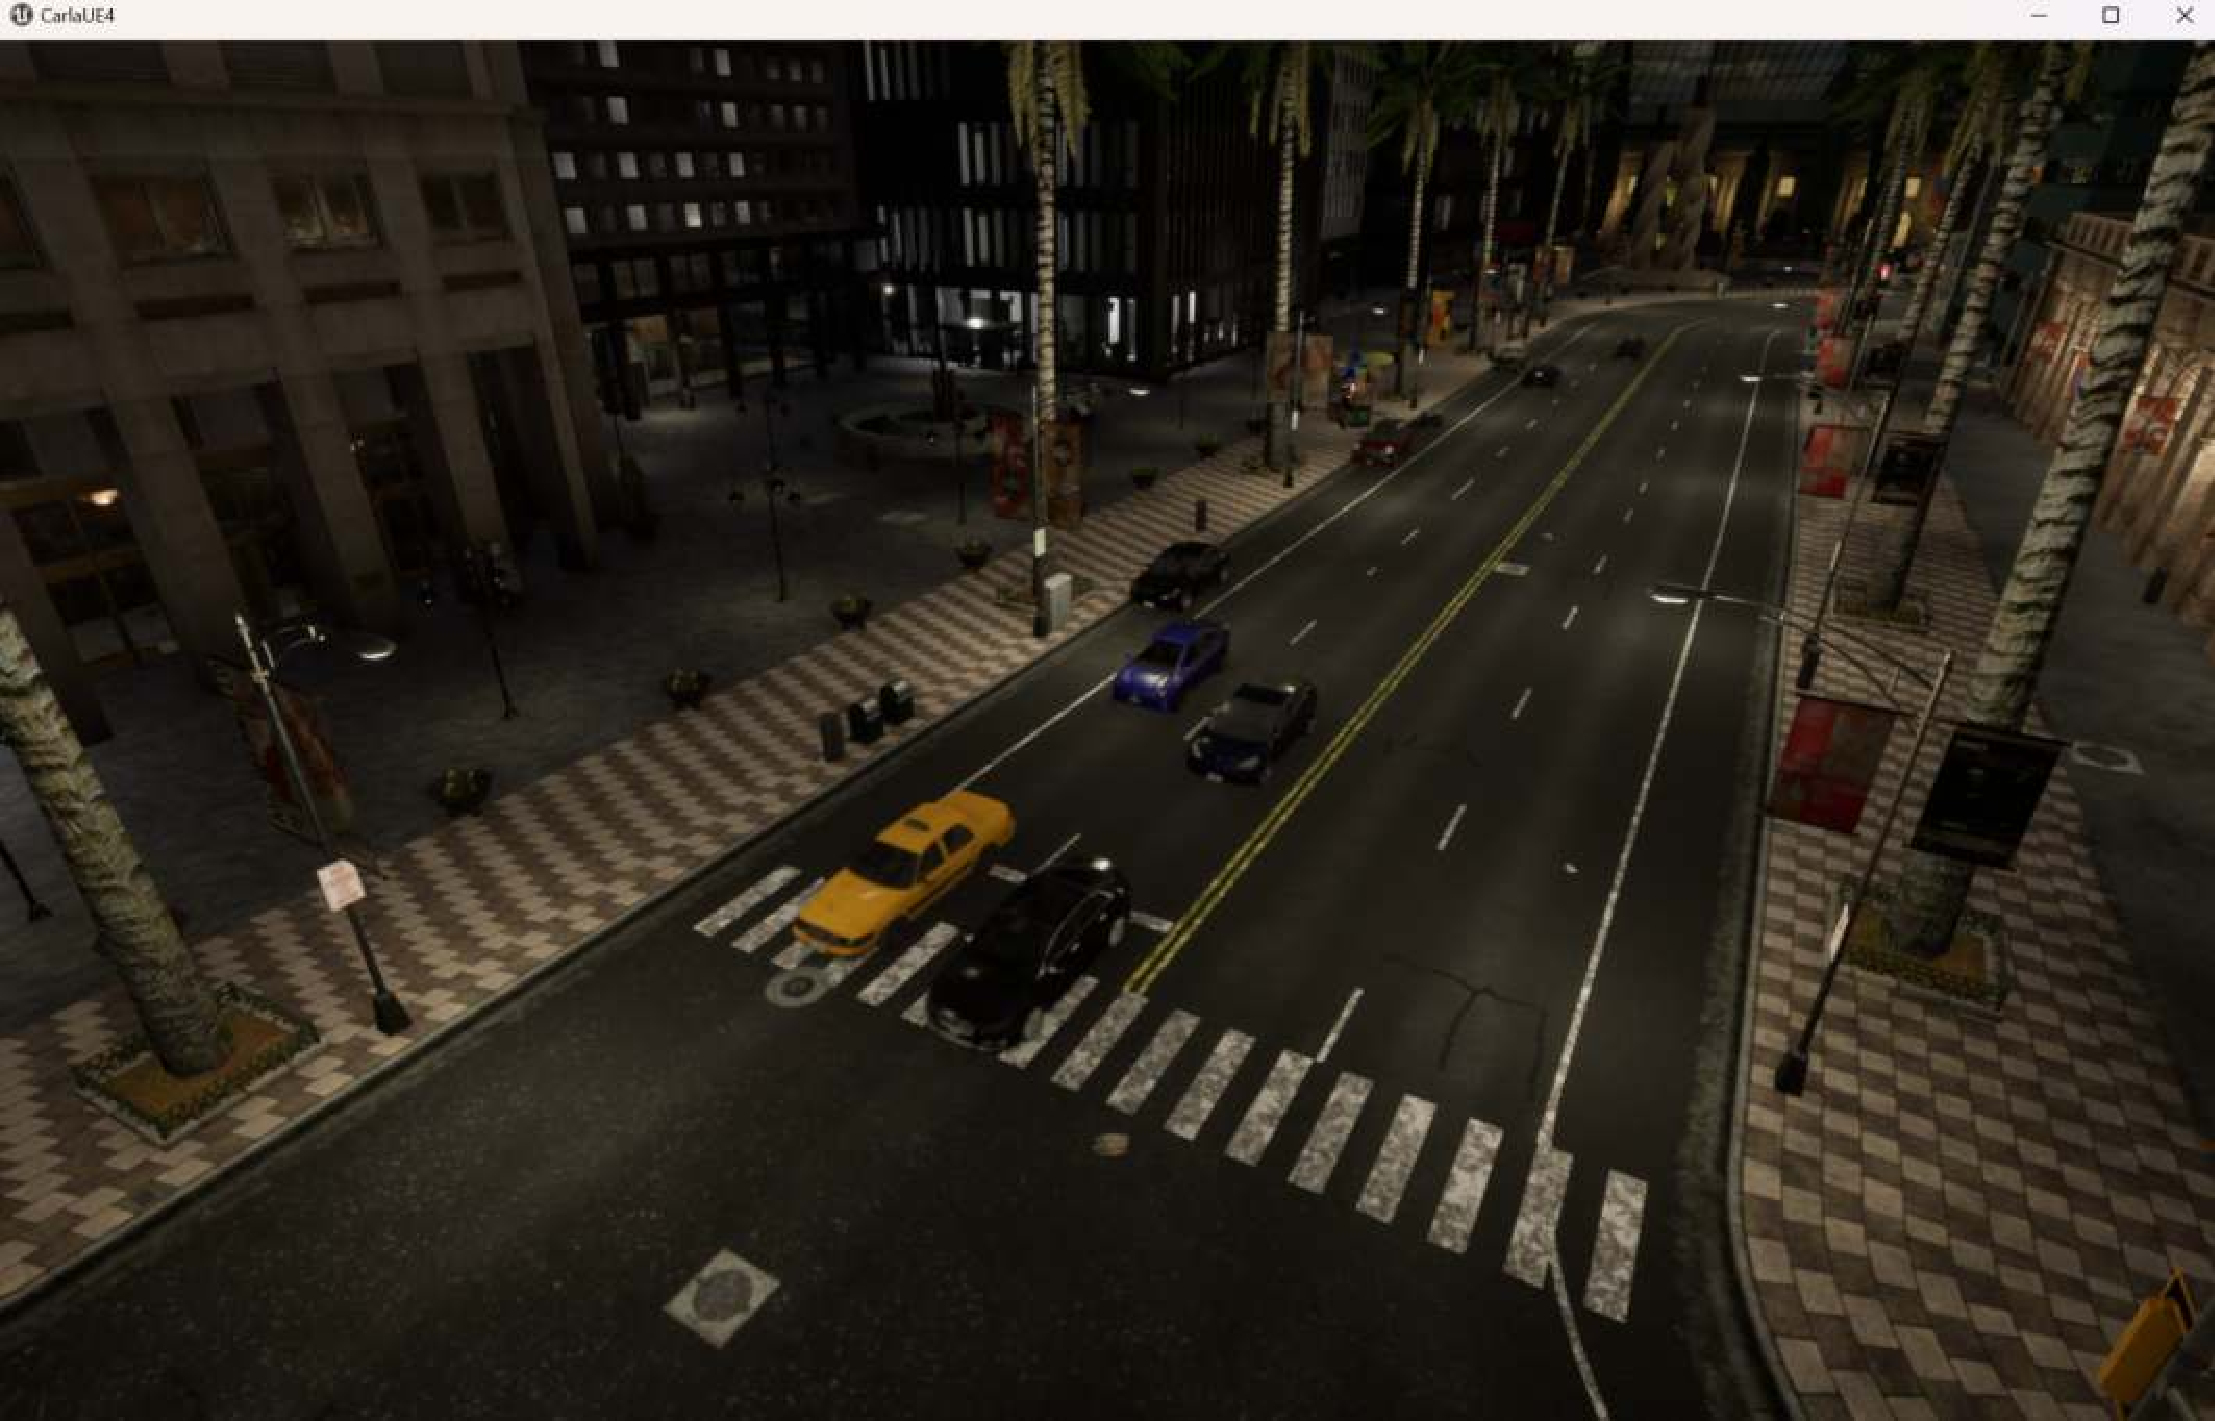
\includegraphics[width=0.7\textwidth]{"images/2.png"}
	\caption{自我车辆在夜晚穿越道路的场景截图}
	\label{fig:night_self_driving_cross}
\end{figure}

\subsection{场景三:自我车辆在夜晚红绿灯前等待信号}
\indent 在夜晚,一些自我车辆在红绿灯前等待信号,而在另一方向,自我车辆正在通行,车灯的光芒穿过昏暗的街道。\\

\begin{figure}[H]
	\centering
	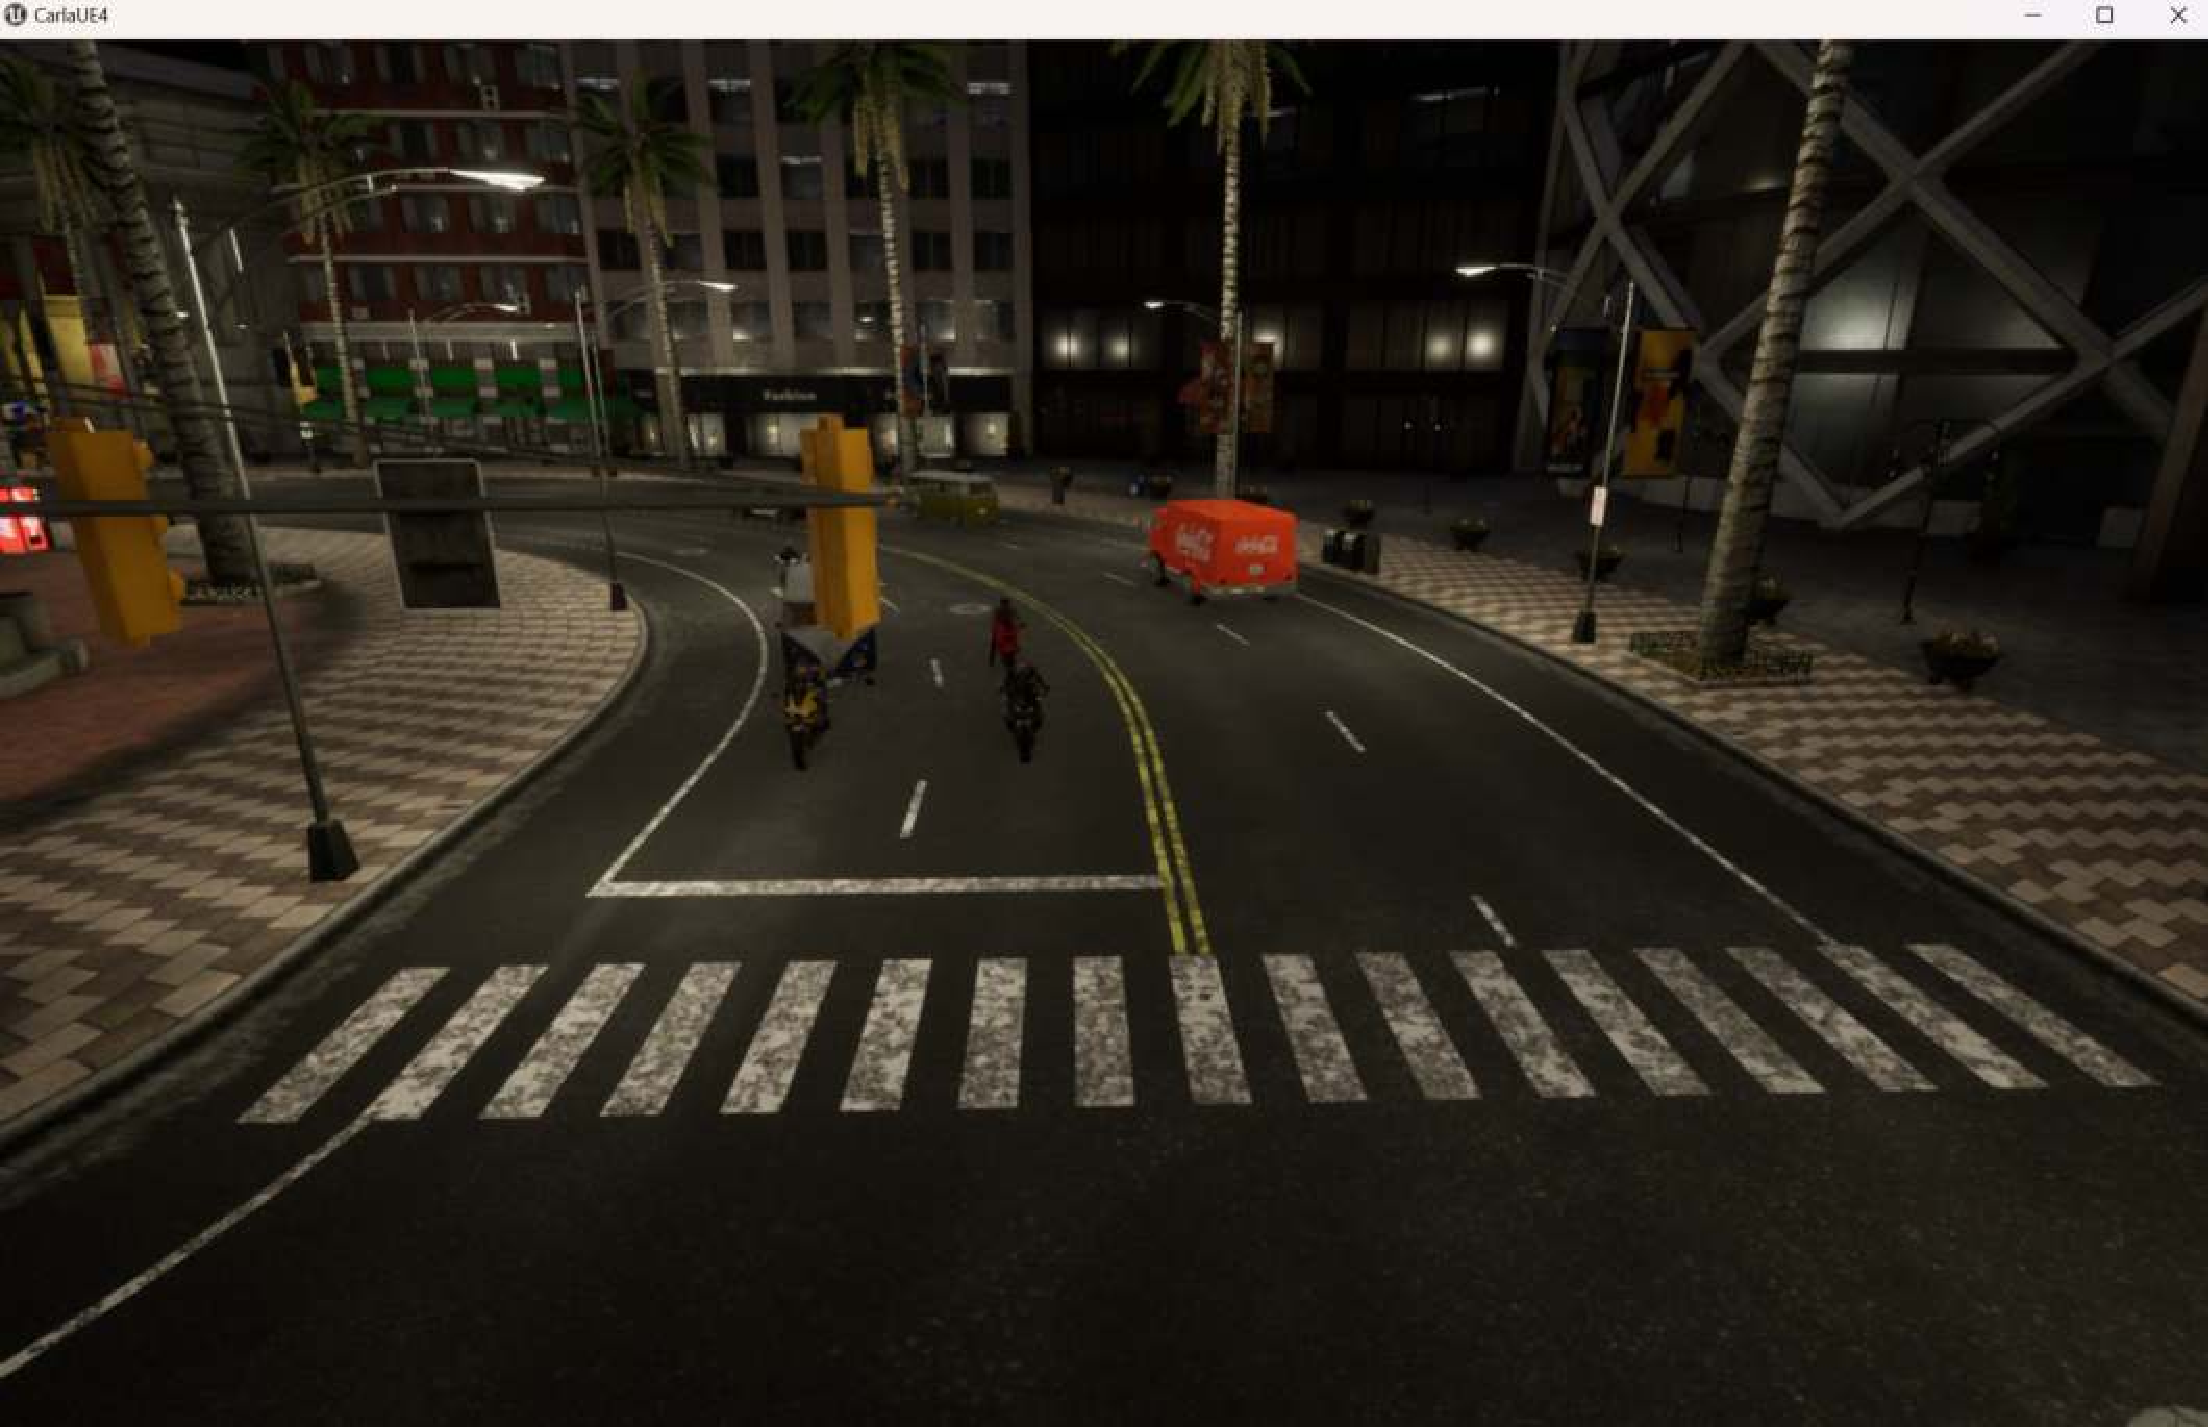
\includegraphics[width=0.7\textwidth]{"images/4.png"}
	\caption{自我车辆在夜晚红绿灯前等待信号的场景截图}
	\label{fig:night_redlight_cross}
\end{figure}

\subsection{场景四:行人横穿直行道路}
\indent 自我车辆在笔直的道路上行驶时,一名行人突然从右前方横穿过来,并在自我车辆接近时突然停下。\\

\begin{figure}[H]
	\centering
	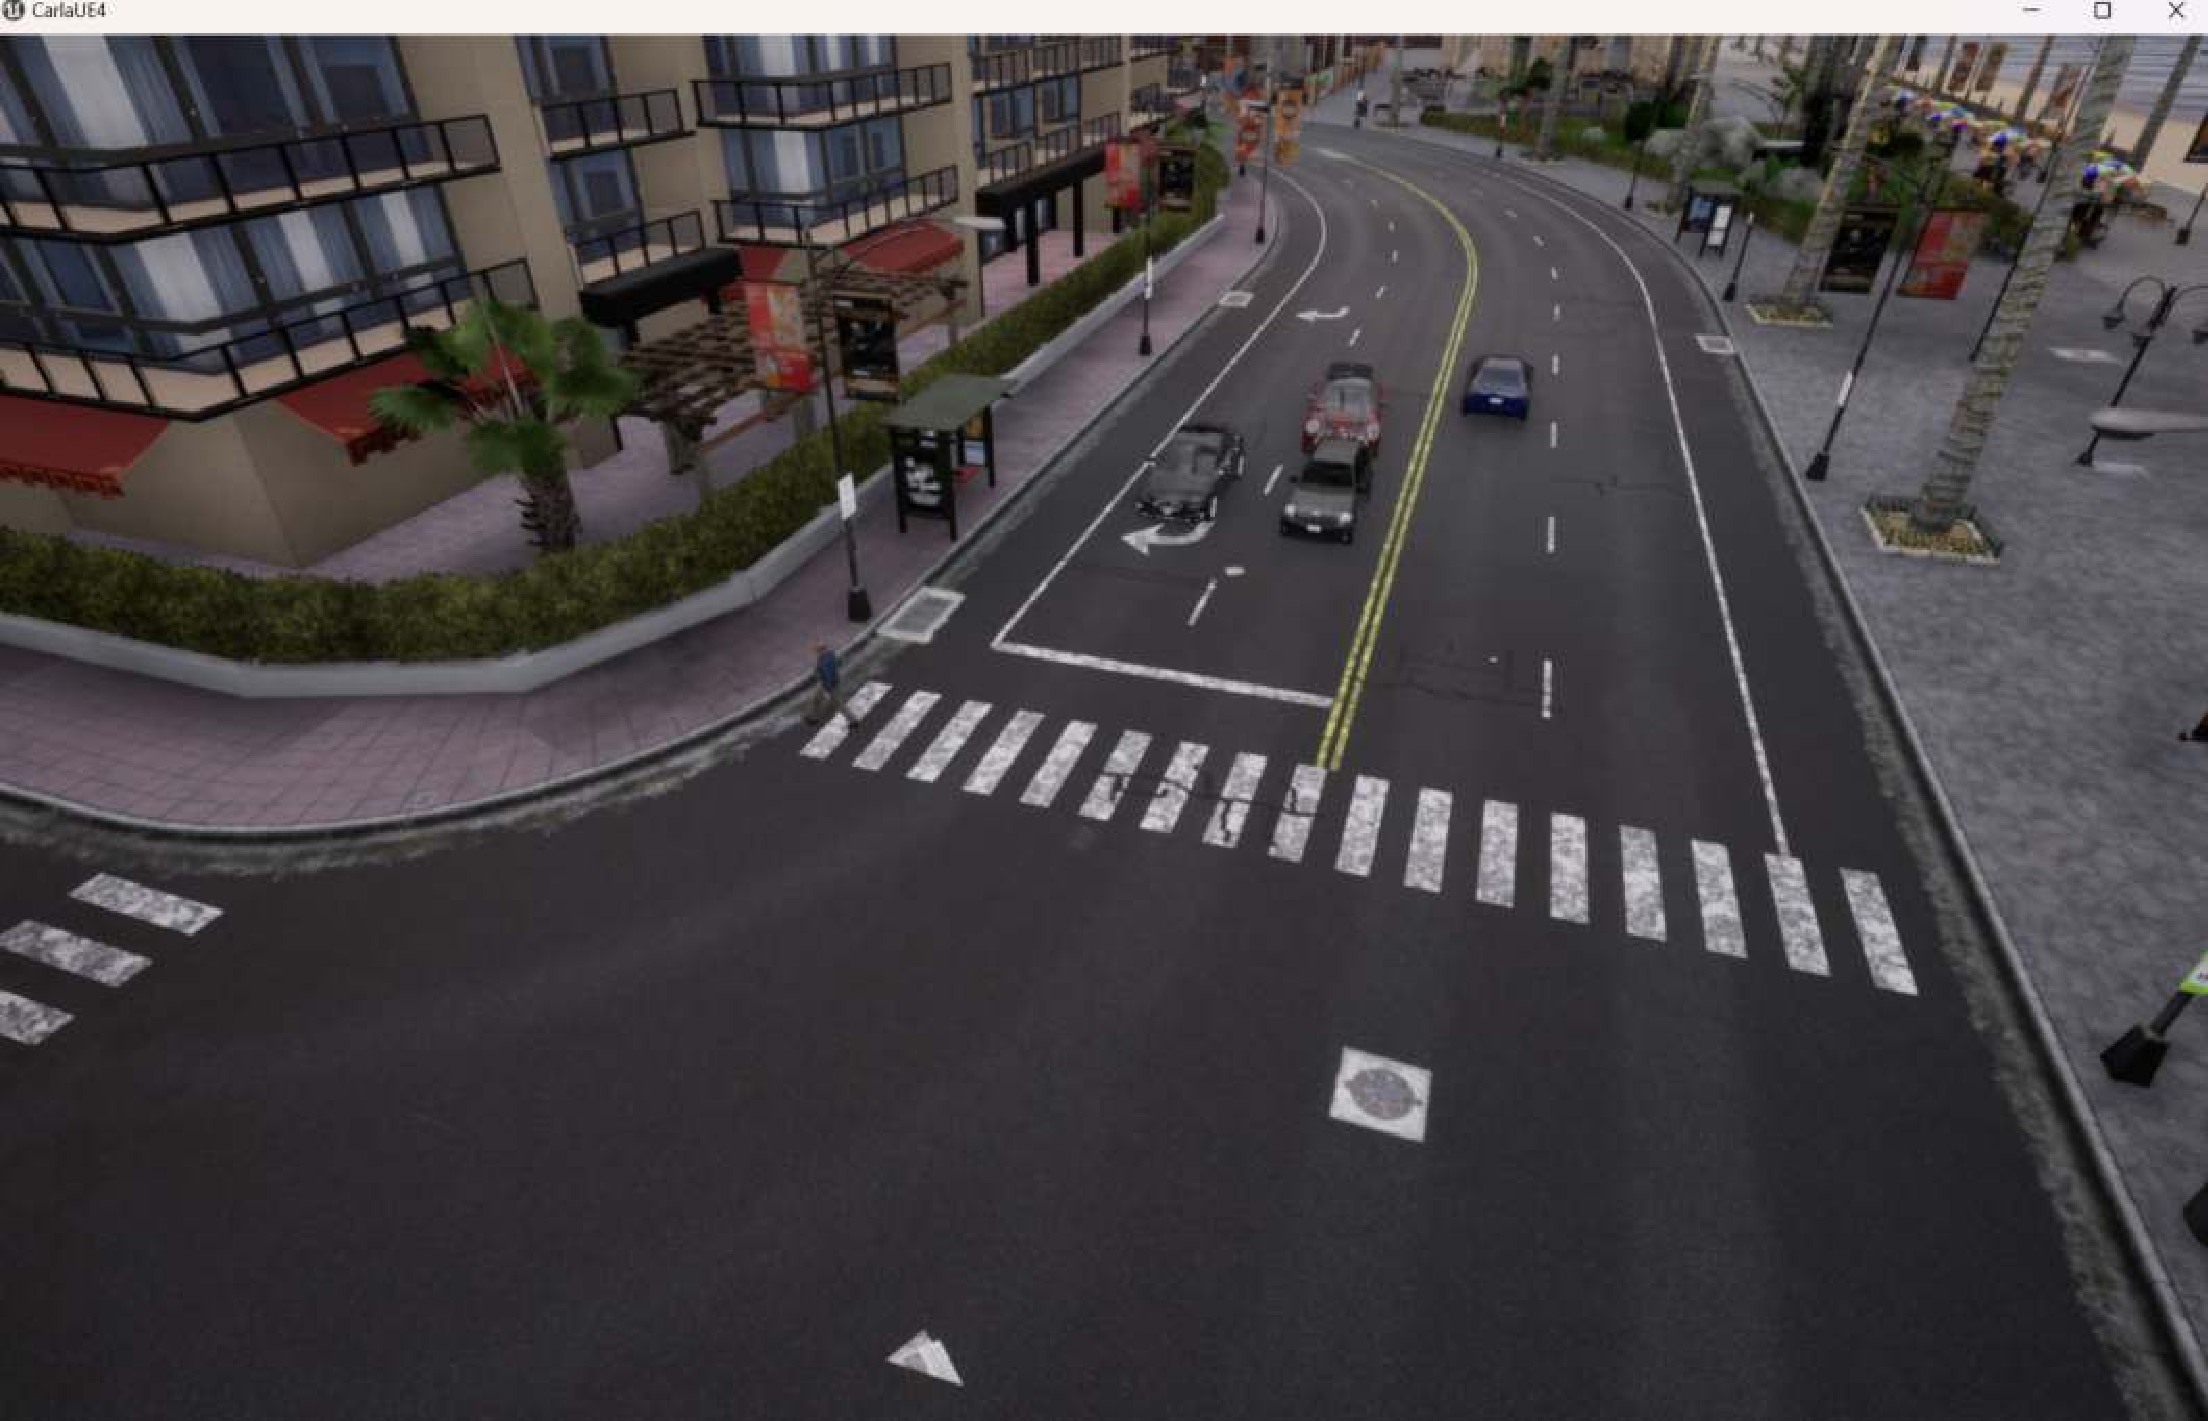
\includegraphics[width=0.7\textwidth]{"images/5.png"}
	\caption{行人横穿直行道路的场景截图}
	\label{fig:pedestrian_crossing}
\end{figure}

\section{实验总结}
本章围绕基于自然语言生成三维交通场景系统的质量验证展开,从评估指标体系的构建、实验设计方法到具体结果分析进行了系统性探讨。针对语义保真度,本文通过构建自动对齐与人工打分机制,验证了系统在理解自然语言输入并准确转化为场景语义元素(如车辆类型、位置关系、动态行为等)方面的能力,实验表明生成场景与自然语言之间的一致性平均达到较高水平,满足语义还原要求。

在场景多样性方面,本文引入结构差异度和行为差异度等量化指标,从宏观与微观两个层面考察系统是否能避免生成模板化、重复性强的场景。通过对多个输入样本批量生成与对比分析,系统展现出良好的生成多样性,能够覆盖多种交通参与者组合、地理位置配置及行为策略,具备服务多样化自动驾驶测试任务的能力。

在效率层面,系统整体运行流程经过优化设计,从自然语言输入到最终仿真场景输出实现端到端的自动化处理。实验统计显示,系统对单条输入的平均响应时间具备稳定性,面对批量输入时也能保持较高的吞吐率,满足现实中高效构建训练数据与仿真环境的需求。

综合来看,本章所提出的评估体系全面覆盖了生成场景的关键质量维度,并通过定量与定性手段相结合的方式,对系统性能进行了客观分析。验证结果不仅证明了系统在自然语言理解、场景构建与高效生成方面的可行性与有效性,也为后续章节中对系统拓展能力的分析与进一步优化方向的提出提供了有力支撑。通过本章的研究,本文为面向智能驾驶系统的高保真场景生成提供了扎实的质量保障基础。